%--------------------------------------------------------------------
\medskip
\subsection{Implementación de modelo multidimensional diseñado en los puntos anteriores}
\label{11}
Para realizar la implementación del modelo multidimensional se ha hecho uso de la herramienta Wizard proporcionada y facilitada en el módulo. Con ella, y basándonos en el modelo lógico descrito en la sección \ref{08}, se ha implementado la implementación del modelo multidimensional que se muestra en la Figura \ref{modelo-multidimensional}.

\begin{figure}[!th]
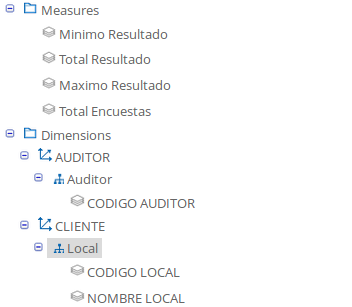
\includegraphics[scale=0.5]{modelo-multidimensional-1.png}
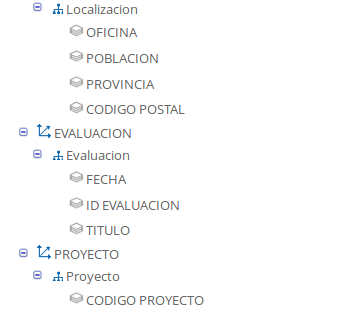
\includegraphics[scale=0.5]{modelo-multidimensional-2.png}
\centering
\caption{Implementación del modelo multidimensional utilizando Wizard.}
\label{modelo-multidimensional}
\end{figure}
